% !TEX root = main.tex
\section{Implementation Steps and Results}
\label{sect:implementation-result}

\subsection{Implementation Steps}
\label{subsect:implementation_steps}
We strictly followed the implementation steps stated in the laboratory manual [3].

\subsection{Code}
\label{subsect:code}

\begin{lstlisting}[language=Matlab]
clc;
clear all;
close all;
D_tr = load('/home/alvi/Documents/courses/ece503/labs/3/data/D_build_tr.mat');
Xtr = D_tr.D_build_tr(1:8,:);
Ytr = D_tr.D_build_tr(9:10, :);
D_te = load('/home/alvi/Documents/courses/ece503/labs/3/data/D_build_te.mat');
Xte = D_te.D_build_te(1:8,:);
Yte = D_te.D_build_te(9:10, :);
Xtr = [Xtr' ones(640, 1)];
I = eye(9);
W_B = pinv(Xtr' * Xtr + 0.01 * I) * Xtr' * Ytr';
W = [W_B(1:8, 1) W_B(1:8, 2)];
b = W_B(9, :)';
e_p = double.empty();
Y = double.empty();
for i=1:128
y = W' * Xte(:, i) + b;
Y = [Y, y];
end
e_p = norm(Yte - Y, 'fro') / norm(Yte, 'fro');
disp(e_p);
I = 1:128;
plot(I, Yte(1, I), 'r', I, Y(1, I), 'g');
plot(I, Yte(2, I), 'r', I, Y(2, I), 'g');
\end{lstlisting}

\subsection{Result}
\label{subsect:result}
\begin{figure}[h]
	\centering
	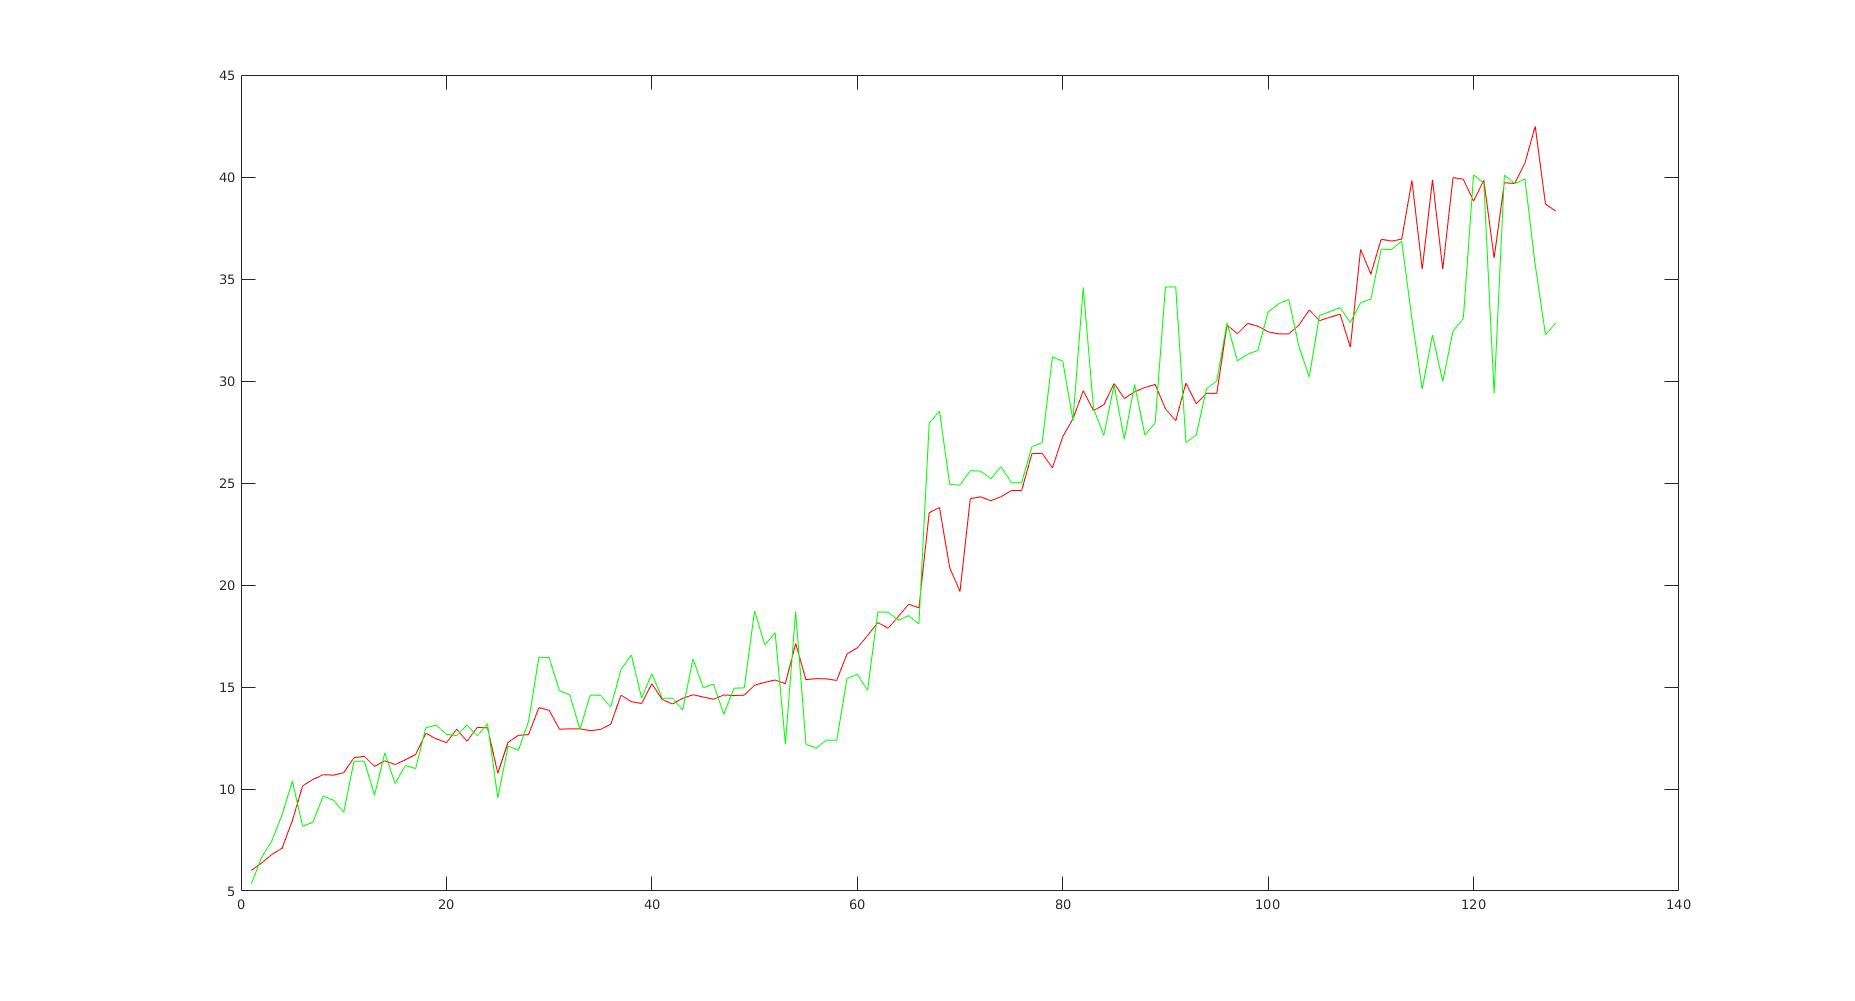
\includegraphics[width=\textwidth]{/home/alvi/Documents/courses/ece503/labs/3/result/1.jpg}
	\caption{First row of $Yte$ and first row of $Y^{(p)}$}
	\label{fig:1}
\end{figure}

\begin{figure}[h]
	\centering
	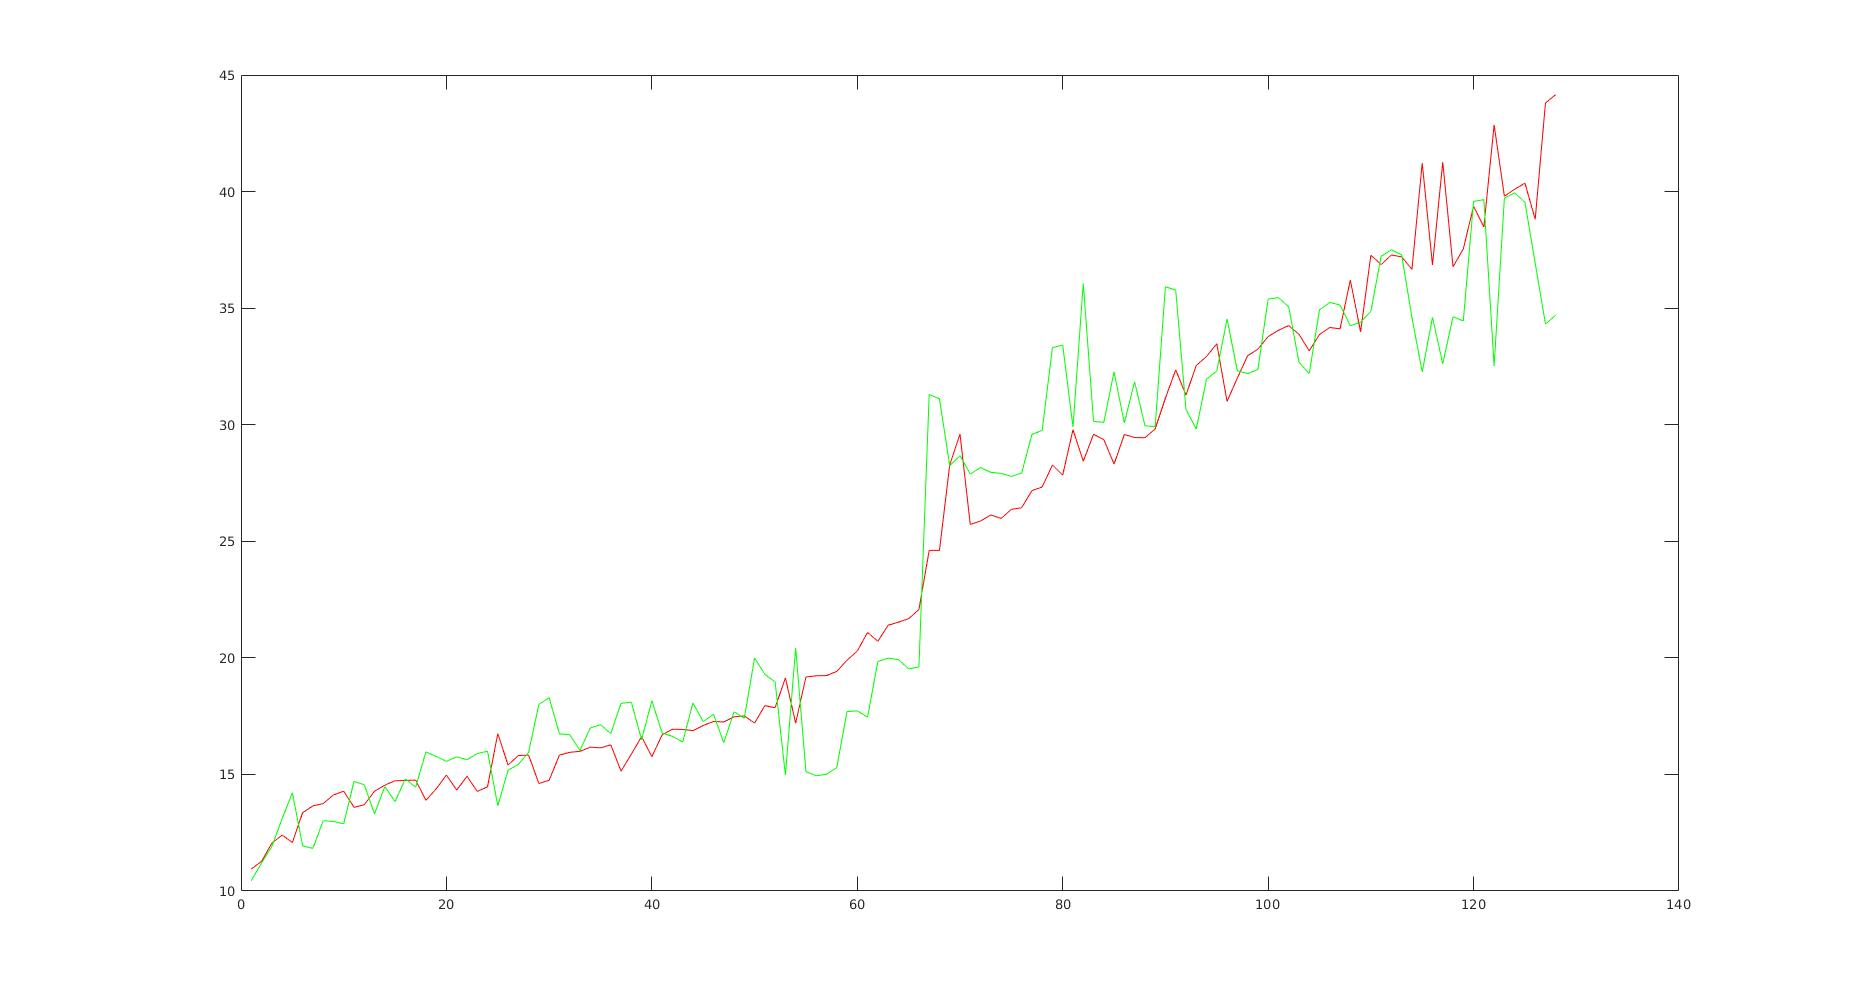
\includegraphics[width=\textwidth]{/home/alvi/Documents/courses/ece503/labs/3/result/2.jpg}
	\caption{Second row of $Yte$ and second row of $Y^{(p)}$}
	\label{fig:1}
\end{figure}